\title{LEZIONE 12 23/04/20}
\textbf{link} \href{https://web.microsoftstream.com/video/55f4d4bd-8efe-48d2-870d-78b0a6baa77d?list=user&userId=cfe0965d-9a7c-40e2-be6e-f078296a1914}{clicca qui}
\section{Client-side scripting}
Lo scripting a lato client è una programmazione focalizzata alla gestione degli eventi prodotti dall'interazione dell'utente.\newline
\newline
Nella versione "thin client" o "pure HTML" il client non fa praticamente nulla: semplicemente invia richeiste, riceve risposte e le mostra a video. Ad ogni evento dell'utente viene ricaricato l'intera interfaccia, si ha una brutta user experience.\newline
\newline
L'architettura "fat client" rende anche il browser un contenitore di funzioni applicative. 
\subsection{eventi}
Nell'architettura "fat client" gli eventi diventano di tre tipi:
\begin{itemize}
    \item trattati solo dal cliente: si cambia l'interfaccia senza senza interpellare il server;
    \item trattati solo dal server: tramite una richiesta HTTP si interpella il server, la cui response sarà la nuova interfaccia, questi sono gli eventi classici dell'architettura "pure HTML";
    \item trattati dal cliente e dal server: il client invia una richiesta HTTP al server, la cui risposta viene usata per modificare parzialmente l'interfaccia.
\end{itemize}
\subsubsection{Eventi "ibridi" gestiti da client e server}
Gli eventi gestiti da client e server permettono di separare l'interazione tra utente e browser da quella tra browser e server (interazione asincrona), tipicamente per:
\begin{itemize}
    \item caricare contenuti dinamicamente;
    \item refreshare dinamicamente contenuti di un interfaccia;
    \item inviare al server un comando senza modificare l'interfaccia utente.
\end{itemize}
La risposta HTTP può produrre l'invio di codice HTML per sostituire una porzione dell'interfaccia, oppure di dati per aggiornare il contenuto dell'interfaccia. E' solitamente preferibile inviare i dati in modo da poter eventualmente usufruire della funzioen anche da applicazioni che non utuilizzano HTML per renderizzare l'interfaccia utente, ma non è sempre così perchè alcune volte calcolare il più possibile a lato server può portare a dei vantaggi.\newline
\newline
In una tipica architettura "pure HTML" si ha un'interazione \textbf{sincrona}. A fronte di un evento che interpella il server, il browser prende il controllo e invia una richeista HTTP e si pone in attesa di una risposta HTTP. In questo periodo di attesa l'utente non può far nulla se non aspettare che la richiesta venga soddisfatta. Quando la riposta arriva il browser ne fa il parsing e ne restituisce un rendering visivo, a questo punto il browser cede nuovamente il controllo all'utente.\newline
\newline
Nell'architettura "fat client" si usano interazioni \textbf{asincrone}. Mentre il browser invia una richiesta HTTP e attende una risposta HTTP, permette comunque all'utente di continuare la sua interazione.\newline
Viene utilizzato il concetto di \textbf{callback}, o chiamata di ritorno, cioè una funzione da chiamare quando un flusso asincrono è giunto termine.\newline
\subsection{Architettura fat client}
Nell'architettura "fat client" viene duplicata la stessa architettura a lato server anche a lato a client.
\begin{center}
    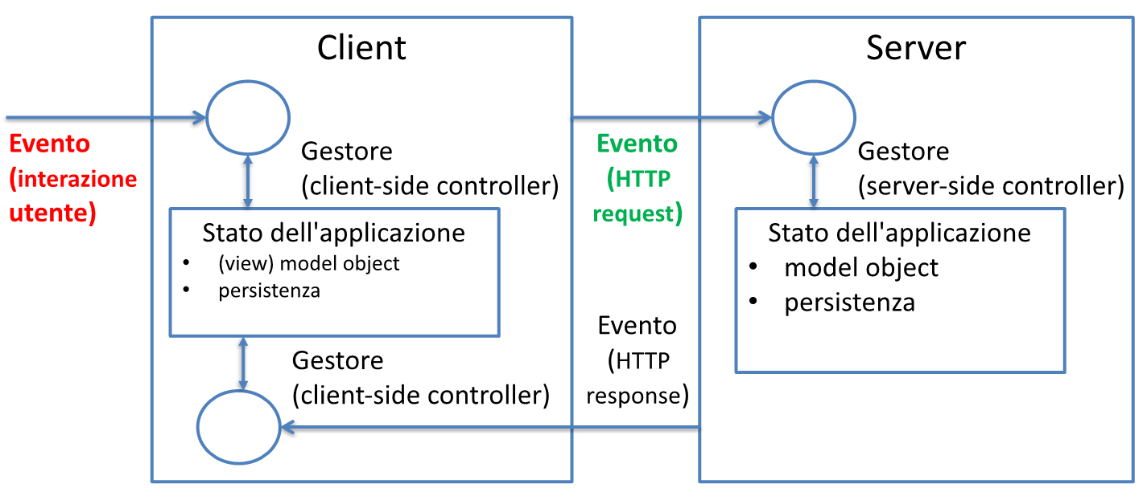
\includegraphics[height=4cm]{../lezione12/img1.PNG}
\end{center}
\subsubsection{Elementi di un'architettura fat client}
\begin{itemize}
    \item Eventi;
    \item Controllore: associa funzion ad eventi;
    \item Stato: stato della presentazione e stato dell'applicazione client.
\end{itemize}
Sorgono quindi nuovi quesiti su come progettare un'applicazione fat client: 
\begin{itemize}
    \item quante view servono?
    \item quali eventi ci sono? dove vengono trattati (client, server, client-server);
    \item dove (in html o javascript) rappresentare lo stato dell'applicazione? dividiamo in stato dell'applicazione e stato dell'interfaccia o farò una cosa sola?
    \item etc\dots
\end{itemize}
Notiamo quindi che ci sono tantissimi modi diversi per progettare un fat client, vediamone due estremi opposti:
\begin{itemize}
    \item Soluzione 1: applicazione a paggine separate e interazioni asincrone per il rinfresco parziale    della vista. Le funzionalità principali sono allocate in pagine diverse, ma vengono usati eventi solo a lato client per gestire eventi che non modificano il contenuto, eventi ibridi server e client vengono usati per gestire eventi che cambiano il contenuto ma non le funzionalità, e eventi che cambiano le funionlità vengono trattati da eventi solo a lato server e il conseguente refresh della pagina.
    \item Soluzione 2: applicazione a pagina singola. Tutte le funzionalità sono realizzate in un unica pagina e tutti gli eventi vengono gestiti almeno a lato client
    \item esistono molte altre soluzioni intermedie a queste due.
\end{itemize}